\chapter{Results}
\paragraph*{}
The Theory chapter \ref{chap:theory} gives a description on how the task of making an image accelerator for edge detection on a gray scale image can be solved. In this chapter test results from implementing the theory on a low budget FPGA \textit{The Xilinx FPGA on the Nexys 3 board} will be presented and discussed.  

\section{Implementation of Sobel operator with extensively extern memory transactions}
\paragraph*{}
The basic design described in section \ref{sec:AccDesign} have been synthesised, simulated and tested on the \textit{Nexys board}. The synthesis report seen in figure \ref{fig:sum_synthesis_report} gives in details how many logic component that have been used to implement the design. This looks seems resonable and looks as expected from the design.  

\begin{figure}[H]
\centering
\begin{BVerbatim}
Summary:
    inferred  31 Adder/Subtractor(s).
    inferred 232 D-type flip-flop(s).
    inferred   3 Comparator(s).
    inferred  59 Multiplexer(s).
    inferred   1 Finite State Machine(s).
\end{BVerbatim}
\caption{Summary of synthesis report ISE project navigator}
\label{fig:sum_synthesis_report}
\end{figure}

\paragraph*{}
Before the design have been implemented on the Nexys board a simulation with ModelSim have been preformed on a image of a roller coaster with $352x288$ pixels see figure \ref{fig:test_picture_raw}. 

\begin{figure}[H]
	\centering
	\begin{subfigure}[b]{0.4\textwidth}
		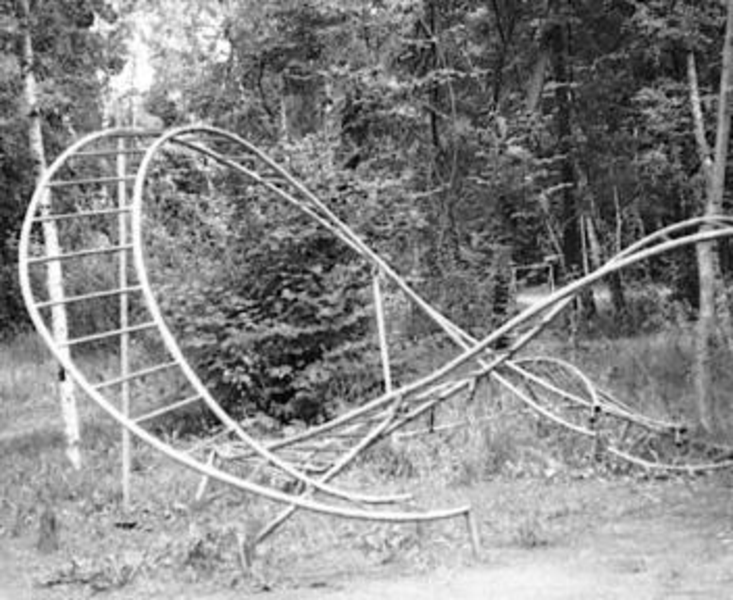
\includegraphics[width=1 \textwidth]{raw.pdf}
		\caption{Raw image before simulation}
		\label{fig:test_picture_raw}
    \end{subfigure}%
        ~ %add desired spacing between images, e. g. ~, \quad, \qquad, \hfill etc. 
    \begin{subfigure}[b]{0.4\textwidth}
    	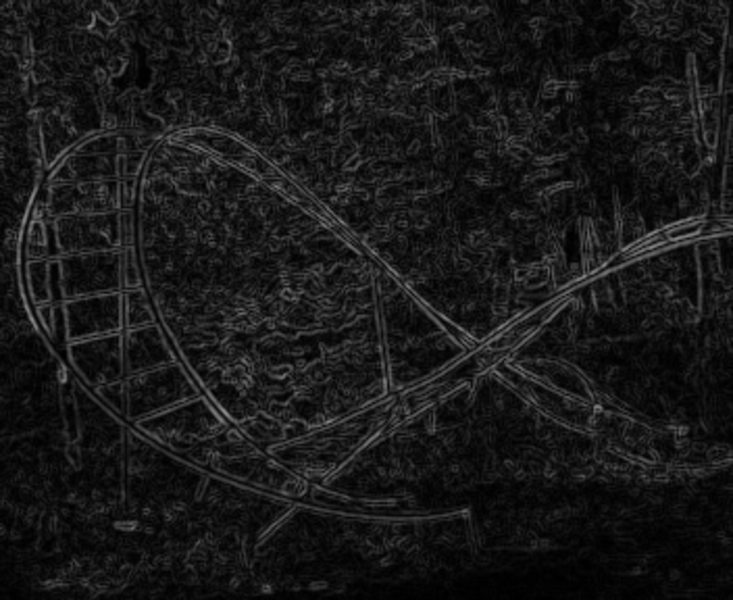
\includegraphics[width=1 \textwidth]{sobel_result.pdf}
    	\caption{After simulation}
    	\label{fig:test_picture_sobel}
	\end{subfigure}
	\caption{Scanline buffering of pixel data.}
\end{figure}

\paragraph*{}
The simulation was completed after $24.4ms$ which result gives a calculation range of $40.9$ $frames~pr.~sec$ or $4.15Mpix/sec$ which is in accordance with the estimations in section \ref{sec:AccDesign}. A section of the waveform from the simulation can be seen in figure ??. The edge detected picture in figure \ref{fig:test_picture_sobel} have been check and verified with the MATLAB verfication script found in appendix \ref{app:Matlab}.   

\section{Optimizations using scanline buffers}
\paragraph*{}
In the section \ref{sec:Optimization} the scanline buffer design was described. As well as with the basic design, the scanline buffer design have been synthesised, tested and implemented. Since this design goes along with the basic design but utilizes a dual block ram the synthesis report gives roughly the same amount of a logic components. See figure \ref{fig:sum_synthesis_report} and \ref{fig:sum_synthesis_report_ram}.   
    
\begin{figure}[H]
\centering
\begin{BVerbatim}
Summary:
    inferred  34 Adder/Subtractor(s).
    inferred 230 D-type flip-flop(s).
    inferred   5 Comparator(s).
    inferred  75 Multiplexer(s).
    inferred   1 Finite State Machine(s).
\end{BVerbatim}
\caption{Summary of synthesis report ISE project navigator}
\label{fig:sum_synthesis_report}
\end{figure}

\begin{figure}[H]
\centering
\begin{BVerbatim}
    DATA_WIDTH = 16
    ADDR_WIDTH = 9
    Found 512x16-bit dual-port RAM <Mram_mem> for signal <mem>.
    Summary:
	inferred   1 RAM(s).
	inferred  32 D-type flip-flop(s).
\end{BVerbatim}
\caption{Summary of synthesis report ISE project navigator}
\label{fig:sum_synthesis_report_ram}
\end{figure}

\paragraph*{}
The simulation of the design have shows the scanline design is improved with only one read transaction per pixel as describe in section \ref{sec:Optimization}. This is proven by the fact the simulation complets after $8.29ms$ which roughly is 3 times faster then the basic design and gives a calculation rate of $120$ \textit{frames pr second} or $12.2Mpix/sec$. As with the basic result the scanline result have been verified with the MATLAB script. In figure ?? a section of the waveform  for the scanline design can be seen.

\section{Optimizations using scanline buffers and bust operation of extern ram}
\paragraph*{}
A further optimization where the extern ram is accessed in burst mode was planed. Some simulation result was obtained but getting a working and verified burst mode optimization within the project time frame have not been possible. In figure \ref{fig:burst_picture} the obtained result is seen the red blobs indicate errors. The problem is that the wait period at every $128word$ reads gives a \textcolor{red}{problem with the pixelbuffers saveing a non exiting pixel this is seen from the image of the errors seen in figure \ref{fig:pic_burst_err}.} is this correct??. The burst optimization was expected to have a calculation rate of $26.7Mpix/sec$ but this is not confirmed by simulation or implementation.
     
\begin{figure}[H]
	\centering
	\begin{subfigure}[b]{0.5\textwidth}
		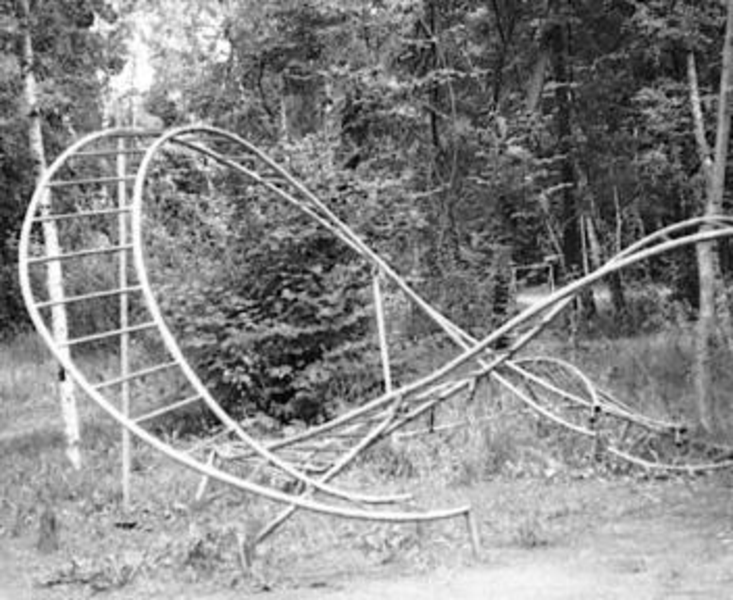
\includegraphics[width=1 \textwidth]{raw.pdf}
		\caption{Raw image before simulation}
		\label{fig:raw_burst}
    \end{subfigure}%
        ~ %add desired spacing between images, e. g. ~, \quad, \qquad, \hfill etc. 
    \begin{subfigure}[b]{0.5\textwidth}
    	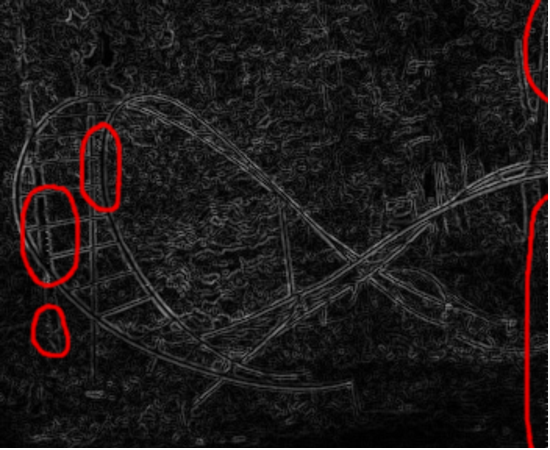
\includegraphics[width=1 \textwidth]{burst_result.pdf}
    	\caption{After simulation red blobs indicated errors}
    	\label{fig:burst_picture_sobel}
	\end{subfigure}
	\caption{Scanline buffering of pixel data.}
    	\label{fig:burst_picture}
\end{figure}


\begin{figure}[H]
	\centering
	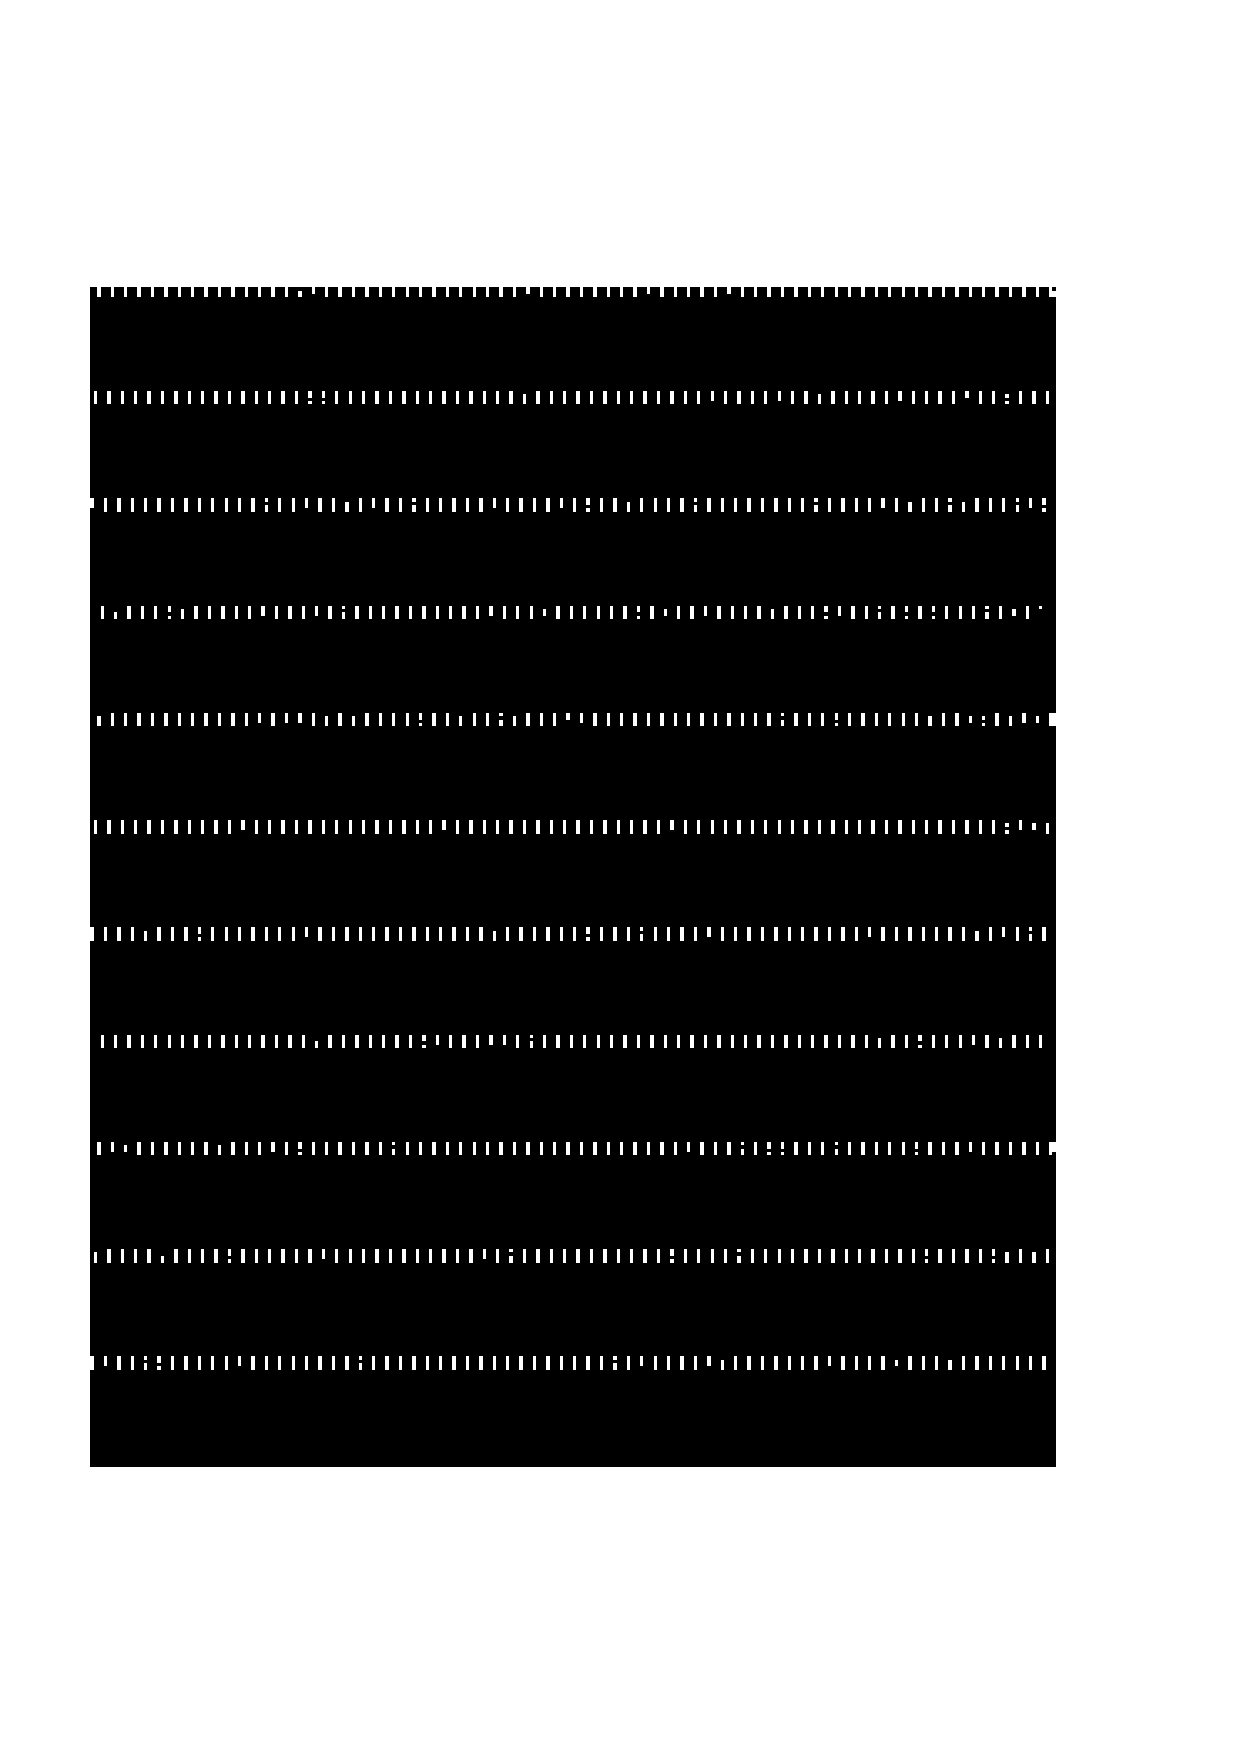
\includegraphics[width=0.5 \textwidth, angle=90]{burst_err.pdf}
	\caption{Image of burst optimization errors}
	\label{fig:pic_burst_err}
\end{figure}